\documentclass[aspectratio=169,11pt]{beamer}
\usepackage[T5]{fontenc}
\usepackage[utf8]{inputenc}
\usepackage[english]{babel}
\usepackage{lmodern}
\usepackage{graphicx,booktabs,tabularx,amsmath}
\usepackage{xcolor}
\graphicspath{{figures/}}

\usetheme{metropolis}
\setbeamertemplate{navigation symbols}{}
\setbeamertemplate{footline}[frame number]

% Same macros as the report
\newcommand{\authorrep}[1]{#1\textsuperscript{\textit{AR}}}
\newcommand{\ours}[1]{#1\textsuperscript{\textit{OUR}}}
\newcommand{\todo}[1]{\textcolor{red}{[TODO: #1]}}

\title{Context-aware ASR}
\subtitle{Survey, Demo and Ablation Study}
\author{Lê Thanh Long \and Trần Quang Hưng \and Lâm Minh Quang \and Bùi Mạnh Hùng}
\institute{VNU-HCM, University of Science -- Faculty of IT\\Speech Processing, Master cohort 35\\Supervisors: Assoc.\ Prof.\ Dr.\ Đinh Điền, Dr.\ Châu Thành Đức, Dr.\ Đỗ Đức Hào}
\date{November 2026}

\begin{document}

\maketitle

\begin{frame}{Outline}
  \tableofcontents
\end{frame}

\begin{frame}{Team and Tasks}
  \small
  \begin{tabularx}{\textwidth}{@{}l X X@{}}
    \toprule
    \textbf{Member} & \textbf{Report/slides} & \textbf{Technical} \\
    \midrule
    Lê Thanh Long & Introduction + Group A & Demo \\
    Trần Quang Hưng & Group B & Demo \\
    Lâm Minh Quang & Group C & Ablation \\
    Bùi Mạnh Hùng & Group D & Ablation \\
    \bottomrule
  \end{tabularx}
  \vspace{4pt}\\ In-depth analysis and proposed improvement: whole team.
\end{frame}

\section{Introduction}
\begin{frame}{Context-aware ASR}
  \begin{itemize}
    \item Plain ASR favours frequent words; names and domain terms are rare in training.
    \item Context (contact list, terms, slides) is given at run time and changes per user, so no retraining.
    \item Goal: fewer errors on listed words, \textbf{without} hurting the rest or inserting listed words that were not said.
  \end{itemize}
  \vspace{4pt}
  \centering\small
  \begin{tabular}{@{}l l@{}}
    \toprule
    Audio says ``call Siobhan'' & Output \\
    \midrule
    Plain ASR & call \textbf{shiv on} \\
    Context-aware & call \textbf{Siobhan} \\
    Over-biased (speaker said ``Sean'') & call \textbf{Siobhan} \\
    \bottomrule
  \end{tabular}\\[4pt]
  {\footnotesize Metrics: WER; B-WER / U-WER = WER on words in / not in the list; false-alarm rate.}
\end{frame}

\begin{frame}{Taxonomy of Approaches}
  \centering
  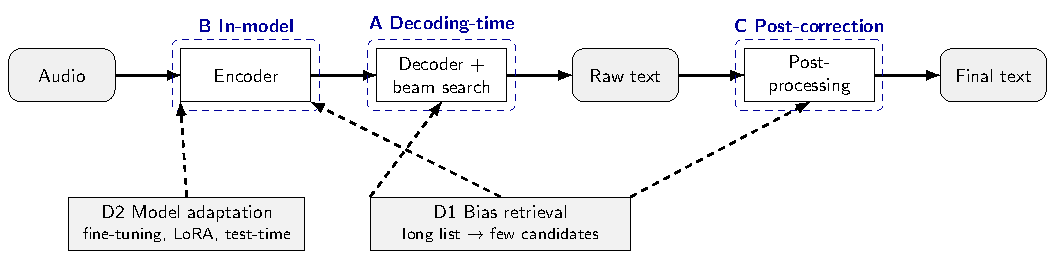
\includegraphics[width=\textwidth]{taxonomy.pdf}\\[4pt]
  \begin{minipage}{.95\textwidth}
    \small
    \textbf{A} bonus score in beam search \quad \textbf{B} list as model input (module or LLM prompt)\\
    \textbf{C} fix errors after recognition \quad \textbf{D1} shrink a long list \quad \textbf{D2} adapt the model
  \end{minipage}
\end{frame}

\section{Survey of Methods}
% One slide per paper; comparison slide at the end of the section
\begin{frame}{Group A: Shallow-Fusion Biasing (Zhao et al., Interspeech 2019, A)}
  \begin{columns}[T]
    \begin{column}{.5\textwidth}
      \textbf{Main idea}
      \begin{itemize}
        \item Bias list $\rightarrow$ contextual WFST; its score is added during beam search.
        \item Bias at \textbf{word-piece} level with weight pushing, so a phrase is not pruned from the beam early.
        \item Activate a phrase only after a context prefix; add proper-noun training data.
      \end{itemize}
    \end{column}
    \begin{column}{.5\textwidth}
      \textbf{Pros / Cons}
      \begin{itemize}
        \item[+] No retraining: swap the list at run time.
        \item[+] Beats a conventional hybrid system on contextual tasks.
        \item[--] Needs a tuned weight $\lambda$ and context prefixes.
        \item[--] Matches spelling, not sound.
      \end{itemize}
    \end{column}
  \end{columns}
\end{frame}

\begin{frame}{Group A: Trie Deep Biasing + Shallow Fusion (Le et al., Interspeech 2021, A)}
  \begin{columns}[T]
    \begin{column}{.5\textwidth}
      \textbf{Main idea}
      \begin{itemize}
        \item Streaming RNN-T with three parts: generic WFST shallow fusion, trie-based deep biasing (joiner), biased NN-LM.
        \item Trie over word pieces gives a binary ``can start / continue a bias word'' vector.
        \item LibriSpeech B-WER (test-clean, $N{=}100$): \authorrep{14.1} $\rightarrow$ \authorrep{5.7}.
      \end{itemize}
    \end{column}
    \begin{column}{.5\textwidth}
      \textbf{Pros / Cons}
      \begin{itemize}
        \item[+] Gains from each part add up; U-WER nearly unchanged.
        \item[+] About 200 MB vs.\ 4 GB for a hybrid baseline.
        \item[--] Deep biasing degrades on lists much longer than in training (400--800 distractors).
        \item[--] Trie biasing alone is weaker than WFST fusion.
      \end{itemize}
    \end{column}
  \end{columns}
  \vfill{\scriptsize AR: author-reported.}
\end{frame}

\begin{frame}{Group B: \todo{CLAS / CopyNE}}\todo{}\end{frame}
\begin{frame}{Group C: \todo{CTC-WS}}\todo{}\end{frame}
\begin{frame}{Group D1: BR-ASR (Interspeech 2025, A)}
  \centering
  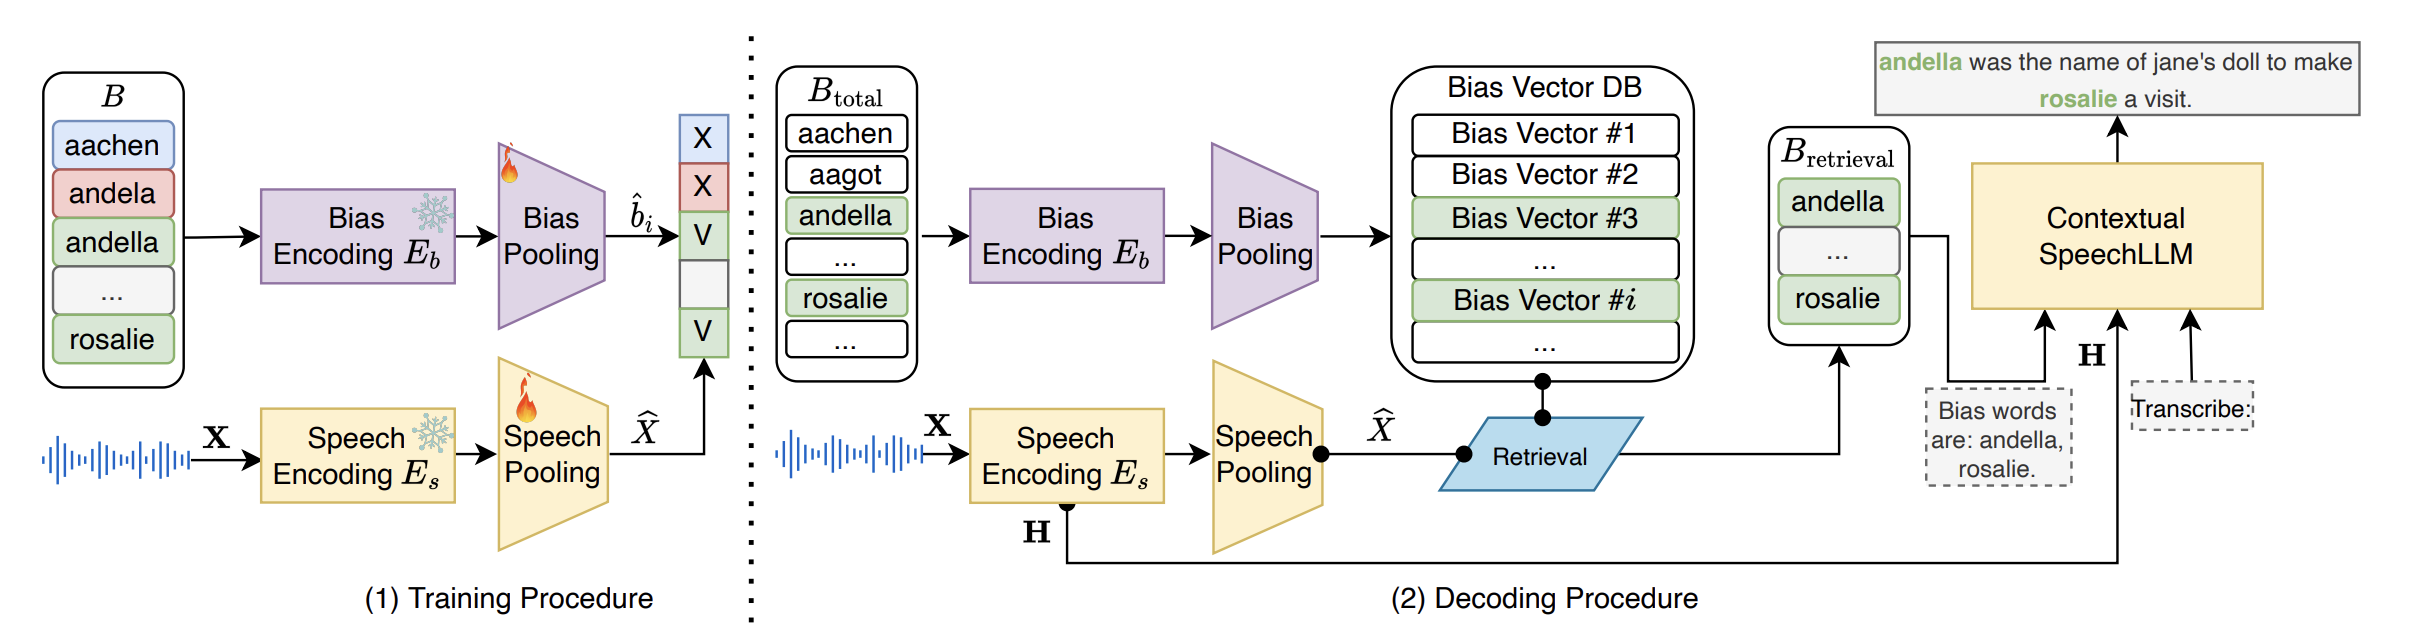
\includegraphics[width=.66\textwidth]{TV4_D1_BR-ASR_pipeline.png}\\[2pt]
  \begin{minipage}{.95\textwidth}
    \footnotesize
    \textbf{Idea.} Retrieve first, then decode: a contrastive retriever picks the top-$K$ bias words from the speech itself, and only these go into the SpeechLLM prompt.\\
    \textbf{Flow.} (1) Train: speech and bias-word vectors in one space, homophone hard negatives; (2) encode the full list once into a FAISS index (up to 200k words);
    (3) per utterance, retrieve the top-$K$ words; (4) the SpeechLLM decodes with ``Bias words are: \dots''.
  \end{minipage}
\end{frame}

\begin{frame}{Group D1: RECAST (EMNLP Findings 2025, A*)}
  \centering
  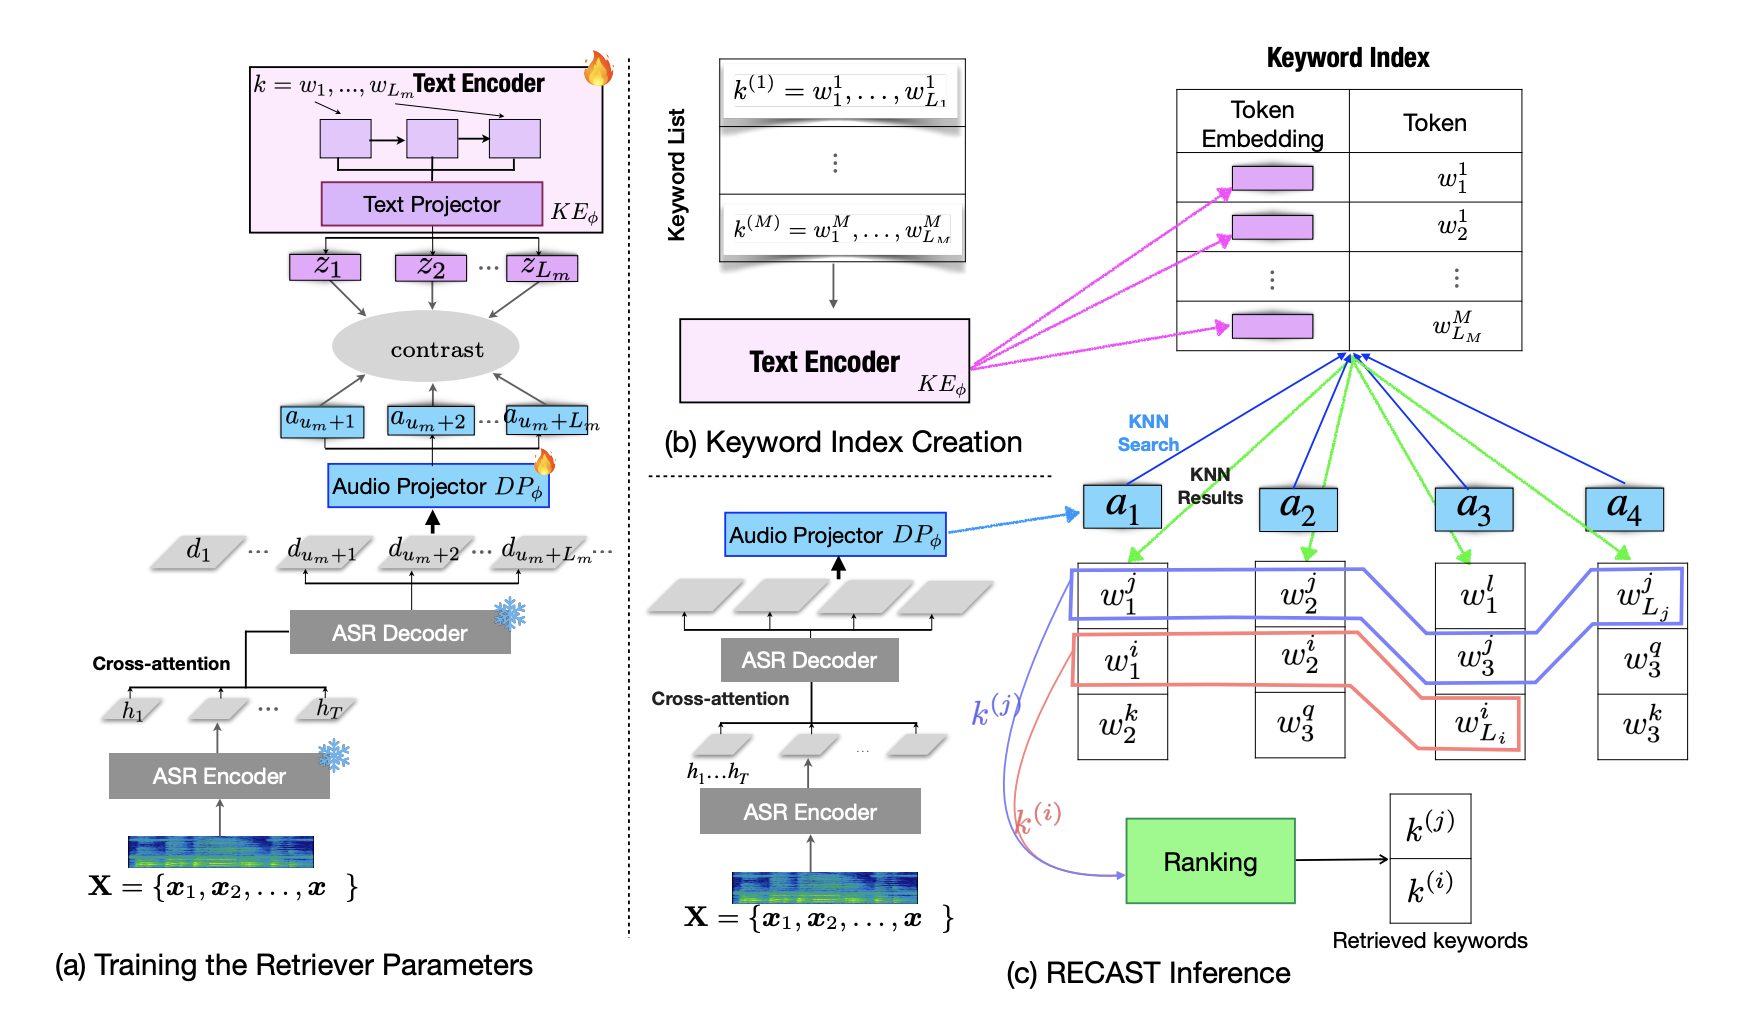
\includegraphics[width=.66\textwidth]{TV4_D1_RECASE_pipeline.png}\\[2pt]
  \begin{minipage}{.95\textwidth}
    \footnotesize
    \textbf{Idea.} Use the decoder state of a frozen Whisper as the query to retrieve keywords; only the top-$\mathcal{K}$ go into the prompt.\\
    \textbf{Flow.} (a) contrastive training of $\mathrm{KE}_\phi$, $\mathrm{DP}_\phi$ (6.5M params); (b) keyword tokens indexed once;
    (c) per step kNN search, token matches chained into keyword spans, then ranked.
  \end{minipage}
\end{frame}

\begin{frame}{Comparison}
  \small
  \begin{tabularx}{\textwidth}{@{}l l l X@{}}
    \toprule
    \textbf{Paper} & \textbf{Group} & \textbf{Venue/Year} & \textbf{Main pros/cons} \\
    \midrule
    \todo{} & & & \\
    \bottomrule
  \end{tabularx}
\end{frame}

\section{Experiments}
\begin{frame}{Demo: Selected Paper}
  \begin{itemize}
    \item \todo{CTC-WS or CopyNE; reason}
    \item \todo{Setup: Colab/Kaggle T4, data}
  \end{itemize}
\end{frame}

\begin{frame}{Demo: Results}
  \centering\small
  \begin{tabular}{@{}l c c c@{}}
    \toprule
    & WER/CER & B-WER / NE-CER & U-WER \\
    \midrule
    Without biasing & \ours{\todo{}} & \ours{\todo{}} & \ours{\todo{}} \\
    With biasing    & \ours{\todo{}} & \ours{\todo{}} & \ours{\todo{}} \\
    Paper         & \authorrep{\todo{}} & \authorrep{\todo{}} & \authorrep{\todo{}} \\
    \bottomrule
  \end{tabular}\\[4pt]
  {\scriptsize AR: author-reported. OUR: our own runs.}
\end{frame}

\begin{frame}{Demo: Qualitative Examples}\todo{reference / baseline / with biasing}\end{frame}

% Ablation is part of Experiments
\begin{frame}{Ablation: Design}
  \small
  \begin{tabularx}{\textwidth}{@{}l X X@{}}
    \toprule
    \textbf{Variable} & \textbf{Values} & \textbf{Metric} \\
    \midrule
    \todo{} & \todo{} & \todo{} \\
    \bottomrule
  \end{tabularx}
\end{frame}

\begin{frame}{Ablation: \todo{variable 1}}\todo{table or figure}\end{frame}
\begin{frame}{Ablation: \todo{variable 2}}\todo{table or figure}\end{frame}
\begin{frame}{Ablation: Discussion}
  \begin{itemize}
    \item \todo{Trade-off B-WER vs U-WER}
    \item \todo{Unexpected results}
  \end{itemize}
\end{frame}

\section{In-depth Analysis}
\begin{frame}{Analyzed Solution}\todo{mechanism, equations}\end{frame}
\begin{frame}{Proposed Improvement}\todo{idea, expected gain}\end{frame}

\section{Conclusion}
\begin{frame}{Conclusion}
  \begin{itemize}
    \item \todo{Contributions}
    \item \todo{Limitations}
    \item \todo{Future work}
  \end{itemize}
\end{frame}

\begin{frame}[standout]Thank you! Questions?\end{frame}

\appendix
\begin{frame}[allowframebreaks]{References}
  \footnotesize\nocite{*}
  \bibliographystyle{unsrt}
  \bibliography{../report/refs}
\end{frame}

\end{document}
